\chapter{Analyse}

\section{Contexte}

\subsection{Présentation du CBMN}

Le laboratoire, créé en janvier 2007, est à l'interface entre le Biologie, la Chimie et la Physique. Il a pour tutelle les départements de Chimie et des Sciences de la Vie du Centre National de la Recherche Scientifique (CNRS) et les Unités de Formation et de Recherche (UFR) de Chimie et de Biologie de l'Université Bordeaux I, II et l'ENITAB. \\
La mission du CBMN est d'apporter une connaissance fondamentale de phénomènes biologiques complexes en les analysant à plusieurs échelles, allant de la molécule à la cellule et à l'organisme. \\
L'équipe ACMPC s'appuie sur deux méthodes d'imagerie : la cryotomographie  électronique et la microscopie à fluorescence. Comme nous l'avons expliqué précédemment, nous allons travailler sur des images issues de cryomicroscopie.  

\subsection{Objectifs}

\noindent
Notre objectif était de créer et d'implémenter une plateforme mettant à disposition plusieurs méthodes de piquage automatisées des particules sur les micrographes. Les échantillons qui nous ont servi de tests étaient de deux types :%
\begin{itemize}
\item des micrographes d'échantillons de virus, de forme ronde, qu'il fallait sélectionner afin de pouvoir déterminer leurs nombre et tailles,
\item des micrographes de protéines membranaires, de forme pyramidale, qu'il fallait aussi sélectionner.\\
\end{itemize}
\noindent
Il était imposé que cette plateforme soit implémentée sous la forme d'un plugin ImageJ. Elle propose à l'utilisateur de se servir des algorithmes de picking pré-installés ou d'en ajouter de nouveaux. Ceci a pour but de simplifier et de centraliser l'accès aux outils de sélection que l'on peut implémenter sur ImageJ.\\%

\noindent
Le logiciel ImageJ a été choisi car c'est un logiciel de traitement et d'analyse d'images développé en \java~\footnote{\java\ est un langage orienté-objet développé par Oracle~\cite{java:url}} par le Nation Institute of Health (NIH).%

\noindent
Ce logiciel est "open-source"~\footnote{son code source est en accès libre et est modifiable(licence GNU-GPL)}, multi-plateforme et bien connu de la communauté scientifique car initialement conçu pour des applications biomédicales. Il s'est peu à peu démocratisé dans d'autres domaines pour sa facilité d'utilisation et les possibilités de développement qu'il offre.%

\noindent
En effet, il est possible de développer soi-même et assez facilement des plugins, que ce soit en \java\ ou en \js ~\footnote{\js est un langage de programmation de script orienté objet à prototype~\cite{javascript:url}}.

\section{\'Etat de l'existant}

\subsection{Détection à l'aide de références}

Cette technique est utilisée pour trouver des particules dans une image en la comparant à un modèle. Celui-ci peut \^etre obtenu soit à partir d'une structure tridimensionnelle connue, soit par sélection d'une particule servant d'exemple dans le micrographe. L'algorithme détermine la meilleure correspondance entre la cible et le modèle pour pouvoir le localiser dans l'image.%

\subsection{Piquage de particules sans références}

\subsubsection{Détection des bords et transformée de Hough}

%$\textcolor{red}{(ref:Automatic Particle Detection Through Efficient Hough Transforms
%by Yuanxin Zhu, Bridget Carragher, Fabrice Mouche, and Clinton S.Potter
%IEEE TRANSACTIONS ON MEDICAL IMAGING,VOL.22,N0.9,September 2003)}$\\


%$\textcolor{red}{(ref:http://en.wikipedia.org/wiki/Hough_transform)}$\\
\paragraph*{}
Les difficultées majeures rencontrées dans les techniques basées sur la détection des contours sont dues à la compléxité de détecter les bords des particules lorsqu'il y a un bruit de fond important sur les images issues de la Microscopie à Transmission Electronique.%

\noindent
Cette technique est basée sur la détection des arêtes ainsi que sur l'application de la transformée de Hough~\cite{PdetectEHT:article}. Cette méthode permet de détecter la présence de formes comme des lignes, des cercles ou encore des ellipses.%

\noindent
Dans la transformée de Hough\cite{HT:url} appliquée à la détection de lignes, pour chaque pixel allumé de l'image on trace toutes les lignes possibles, on obtient alors une sinusoïde unique appelée espace de Hough. Si les courbes associées à deux points se coupent, l'endroit où elles se coupent dans l'espace de Hough correspond aux paramètres d'une droite qui relie ces deux points (ordonnée à l'origine et pente).%

\paragraph*{}
La détection de formes s’apparentant à des cercles ou des axes circulaires se fait en détectant le centre de celles-ci.
Pour chaque pixel allumé, la fonction trace un cercle de rayon donné. Si la forme a le même rayon que le cercle tracé, tous les cercles se recoupent au centre de la forme, on constate ainsi une amplification de la valeur du pixel central.

\paragraph*{}
D'autre part, pour détecter des particules de formes irrégulières, l'approche décrite précédemment peut également \^etre utilisée mais la transformée de Hough devra alors \^etre remplacée par la transformée de Hough Généralisée~\cite{GHT:url}.
Cette nouvelle méthode repose sur la modification de la transformée de Hough en utilisant le principe de l'identification à partir d'un modèle de référence.
%$\textcolor{red}{(ref:http://en.wikipedia.org/wiki/Generalised_Hough_transform)}$\\

\subsubsection{DoGLFC et classement par affinité}

%$\textcolor{red}{(ref: Reference-free particle selection enhanced with semi-supervised machine learning for cryo-electron microscopy
%by Robert Langlois, Jesper Pallesen, Joachim Frank
%Journal of Structural Biology 175, (2011)353-361)}$
\paragraph*{}
Cette technique est basée sur l'utilisation de l'algorithme DoGLFC\footnote{Difference Of Gaussian Local Fast Correlation} complété par l'algorithme de classement par affinité~\cite{DoGAff:article}.

\paragraph*{}
Le DoGLFC est basé sur l'algorithme DoG Picker du Scripps Institute\cite{Scripps:url}, une méthode rapide qui permet la segmentation de particules. Après l'application de l'algorithme de Différence de Gauss (DoG), on obtient une cartographie de points similaire à celle de la méthode utilisant un modèle de référence.%\blue {\Large ?!} \black %

\noindent
Cet algorithme requiert un paramètre ajustable unique ou un jeu de paramètres basé sur le rayon de la particule ou un ordre de grandeur du rayon. L'exécution de cet algorithme renvoie une liste de trois paramètres décrivant la localisation de la particule (les coordonnées \emph{x} et \emph{y}) et la taille du pic.%

\noindent
L'algorithme DoGLFC sélectionne les particules (ou objets) potentielles de taille déterminée, ceci a un pouvoir discriminatif moindre par rapport à une technique basée sur un modèle de référence.

\paragraph*{}
Pour améliorer le rendement lors du piquage des particules, un nouvel algorithme semi-supervisé, le classement par affinité, peut \^etre appliqué.

\noindent
L’algorithme a besoin de trois paramètres d'entrée: un jeu d'images, la taille minimale de l'image après réduction et deux références indiquant quelle fen\^etre doit \^etre utilisée comme référence positive ou négative.

\noindent
Lorsque l'algorithme a fini de se dérouler, on obtient une classement pour chaque fen\^etre où le maximum correspond à la particule ciblée.

\paragraph*{}
L'utilisation de DoGLFC complété par le classement par affinité permet d'extraire
rapidement les particules de l'image et d'éliminer avec précision les particules correspondant à de la contamination ou du bruit de fond.

\subsection{Perceptron}

\paragraph*{}
Un perceptron est une sorte de réseau neuronal artificiel. Dans son état le plus simple, il représente un système de classification binaire/linéaire.%

\noindent
Ce programme a la particularité d'être capable d'apprendre des concepts, ce qui signifie qu'il peut apprendre afin de répondre par vrai ou faux à des données qui lui sont soumises, gr\^ace à la présentation répétée de plusieurs exemples d'étude.
Il a déjà été testé sur des images binaires pour la détection de formes ou de contours mais pas sur des images en niveaux de gris ou sur des problèmes de reconnaissance de modèles visant à sélectionner des particules. Le réseau neuronal n'a pas non plus été exploité comme un outils de sélection automatique de particules mais plusieurs recherches ont conclu qu'il pourrait \^etre utilisé pour l'élimination de faux-positifs.~\cite{Perceptron:article}.%

\section{Analyse des besoins}

\noindent
Ils sont de deux types: fonctionnels et non fonctionnels, et diffèrent entre l'interface utilisateur et les algorithmes de piquage.

\subsection{Besoins fonctionnels}

\subsubsection{Interface}

\noindent
Au lancement, les images sont préalablement chargées sur \imj , l'utilisateur a le choix entre plusieurs algorithmes de picking. %L'interface propose un mode de prévisualisation afin de vérifier le piquage sur une image avant de l'appliquer au stack entier.
Nous avons essayé de faire en sorte que l'affichage soit clair et succinct, constitué d'un menu déroulant, d'une liste de boutons et d'une interface propre à chaque algorithme.\\
Enfin, il est également possible d'implanter simplement de nouveaux algorithmes dans l'interface. % Simplement, ou pas ^^

\subsubsection{Les algorithmes}

Ils réalisent un piquage automatique des particules depuis les micrographes issus de \cme. Le format de sortie est un tableau de résultats contenant un jeu de coordonnées \emph{x, y} associé à la position de l'image dans le stack, ainsi qu'un mini-stack contenant les particules sélectionnées par l'algorithme si l'utilisateur le désire.

\subsection{Besoins non fonctionnels}

\subsubsection{Interface}

\noindent
L'implémentation de la plateforme a été réalisée en \java, nous utilisons les API\footnote{Application Programming Interface} graphiques de la bibliothèque \emph{Swing}. 
Il s'agit d'une interface graphique (GUI)\footnote{Graphic User Interface} faisant partie du paquage Java Foundation Classes (JFC), inclus dans J2SE. Swing constitue une des principales évolutions apportées par Java2 par rapport aux versions antérieures. Elle offre la possibilité de créer des interfaces graphiques identiques quelque soit de système d'exploitation sous-jacent, au prix de performances moindres qu'en utilisant Abstract Window Toolkit (AWT) l'autre bibliothèque principale pour \java. \\
De plus, nous avons essayé de faire en sorte que le programme soit le plus simple d'utilisation possible afin de le rendre accessible à tous. C'est pourquoi nous avons tenté de faire un code clair, explicite et commenté afin de permettre aisément l'implémentation de nouveaux algorithmes.

\subsubsection{Les algorithmes}

\noindent
Les algorithmes ont été testés avec l'outil macro d' \imj ~puis implémentés en \java, nous avons fait en sorte que le temps de déroulement de l'algorihtme soit assez rapide afin de pouvoir gérer de grands jeux de données et qu'aucune image de traitement intermédiaire n'apparaisse à l'utilisateur (à moins qu'il ne le souhaite).\\

Dans l'optique de démocratiser l'utilisation de notre interface et afin de permettre l'extension de ce plugin avec d'autres algorithmes, le projet a été placé sous une licence GPL\footnote{General Public License~\cite{GPL:url}}.

\noindent
%Le projet devra être terminé vers mi-mai. %prière de nous mettre une bonne note !

\section{Scénario d'utilisation du plugin}

Nous prenons l'exemple d'une image issue de \cme ~sur laquelle se trouvent des protéines membranaires que nous voulons sélectionner (Figure \ref{prot}).

\begin{figure}[h] 
\begin{center}
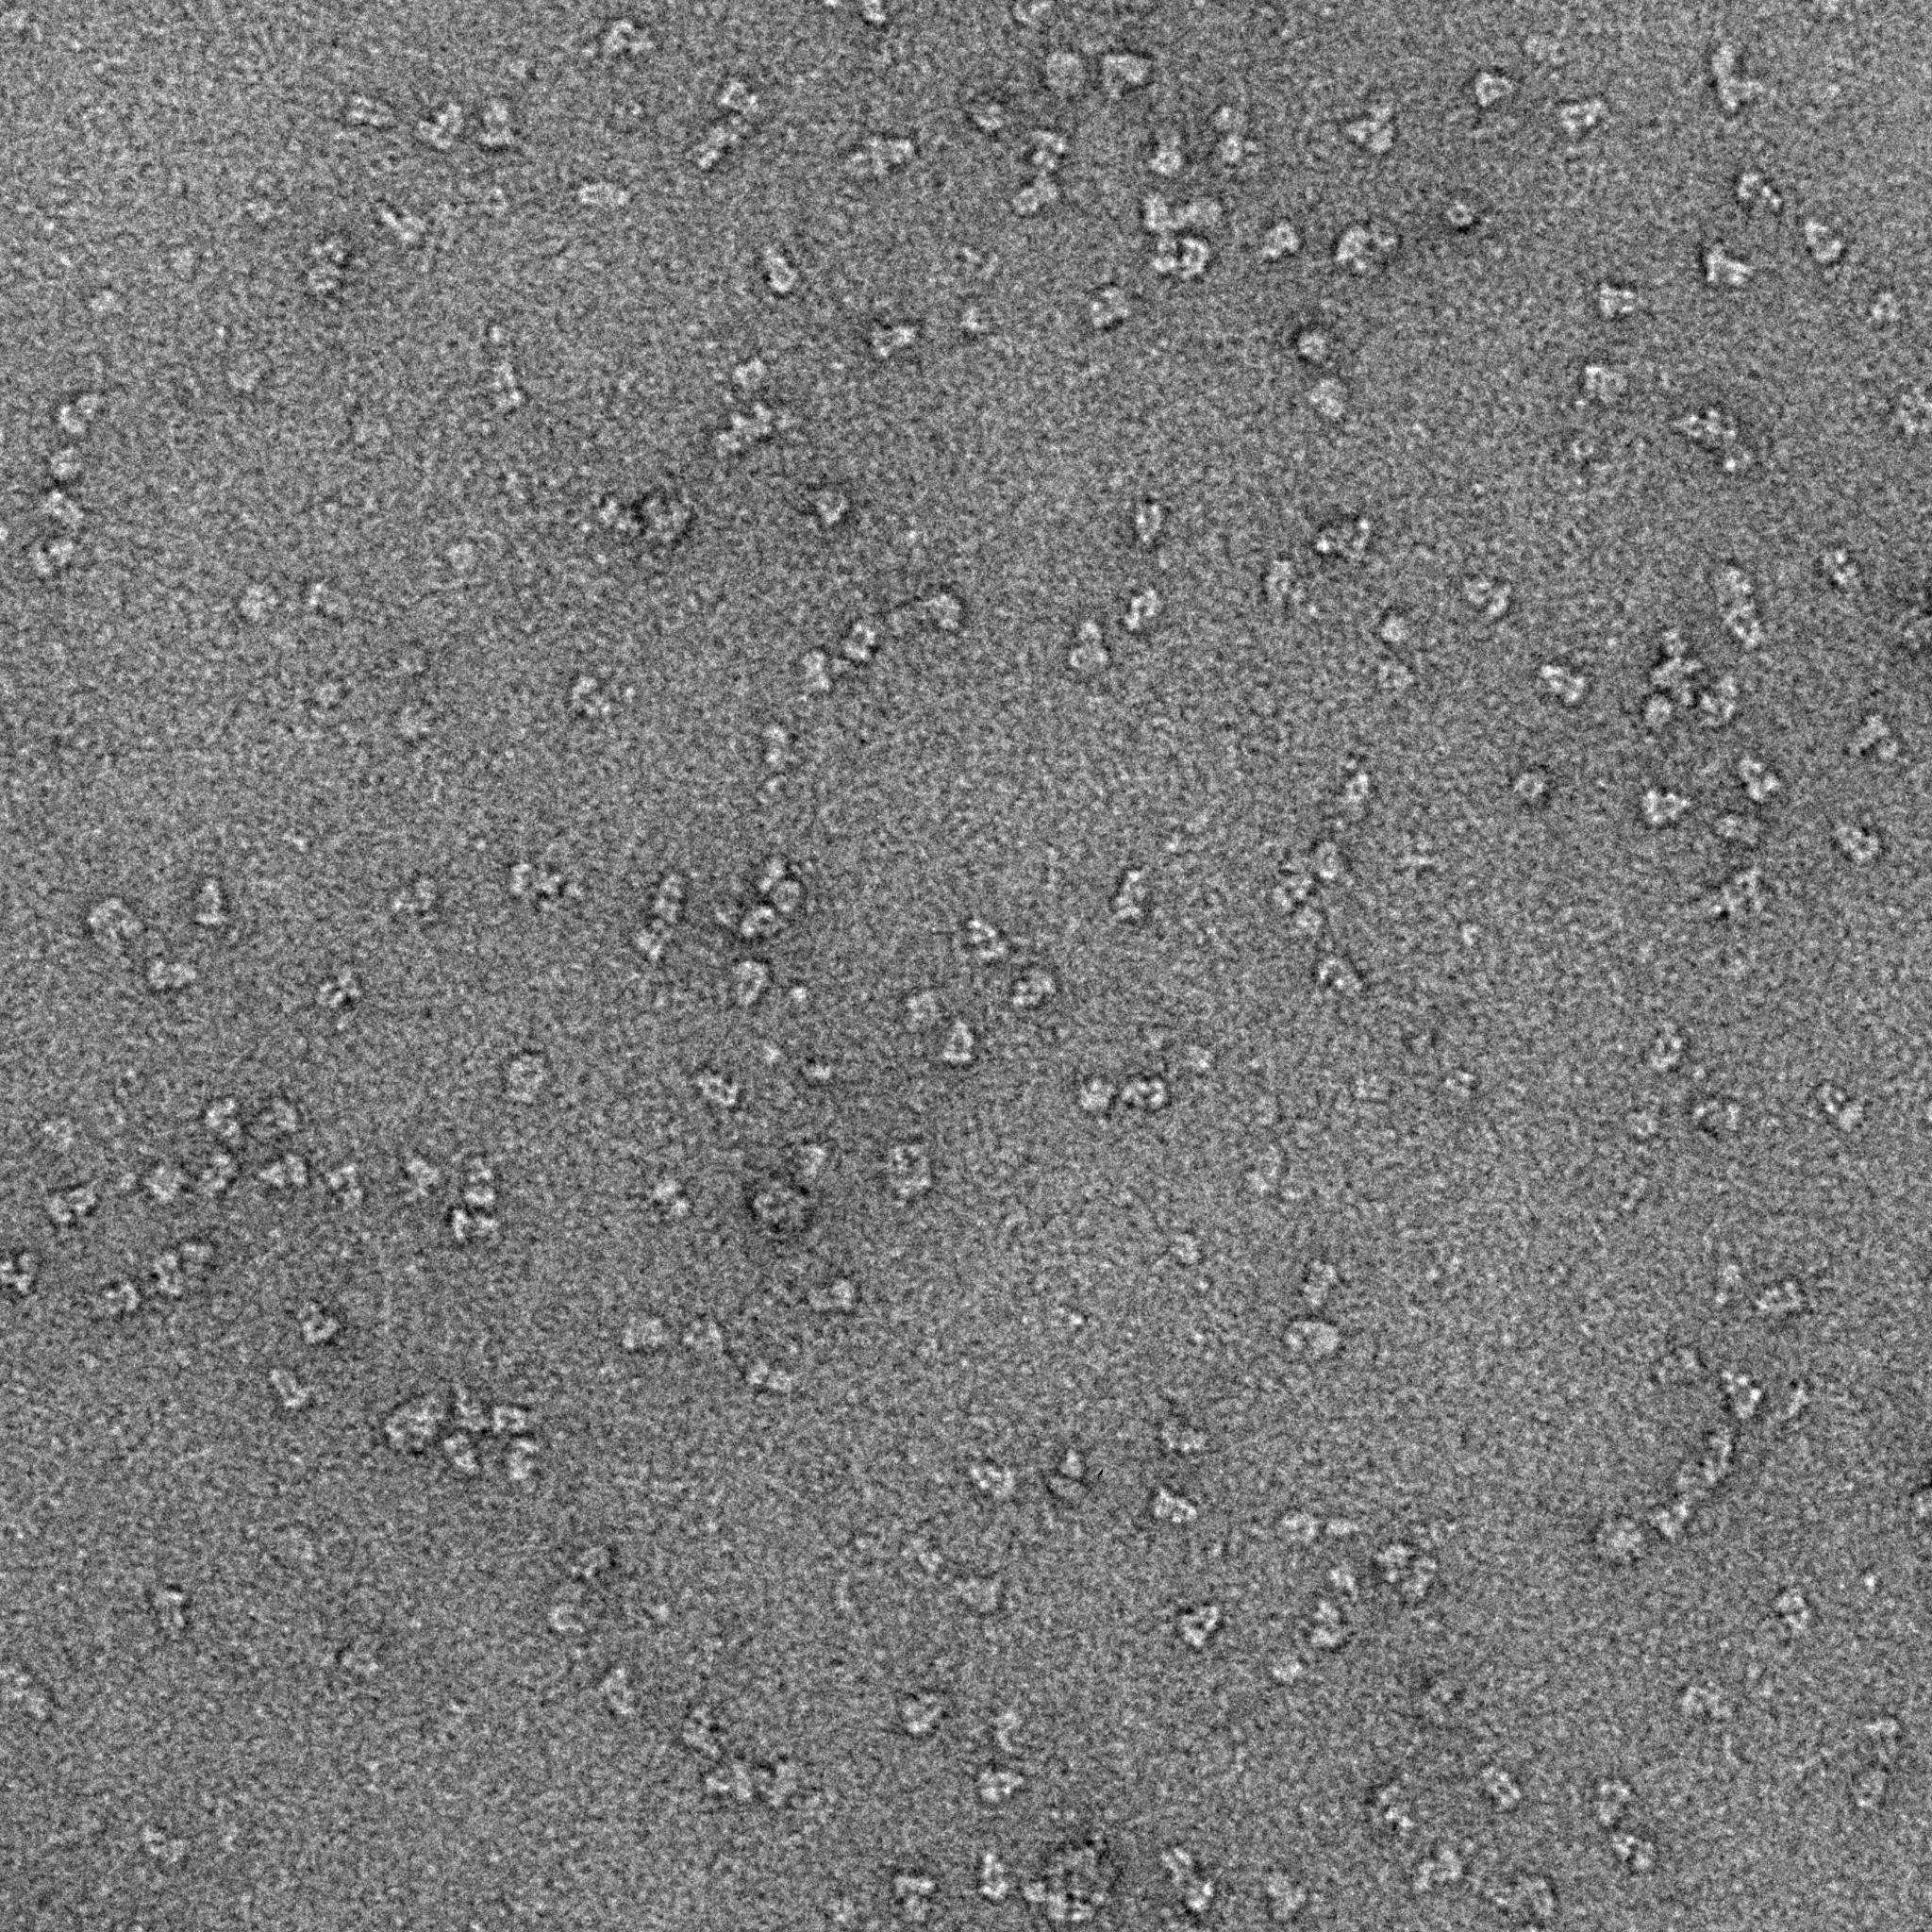
\includegraphics[width=0.5\textwidth]{proteines.jpg}
\caption{Image de protéines membranaires observées au \cme}
\label{prot}
\end{center}
\end{figure}

Nous avons tenté de nous mettre à la place d'un chercheur pour avoir une vision biologique de l'utilisation de notre plugin. Tout au long de ce rapport, vous pourrez donc suivre toutes les procédures qui nous ont permis de réaliser la sélection. 













